% La siguiente seccion enmarca el contexto
% que envuelve al proyecto y de alguna
% manera el por qué
\section{Contexto}

Hoy en día se tiende a tener distintos recursos de cómputo en un solo dispositivo, por ejemplo, en un teléfono móvil ya tenemos al menos un procesador y una tarjeta gráfica, pero no tan sólo en el ámbito más cotidiano (aunque no nos demos cuenta), sino que en los más profesionales y especializados está siendo también cada vez más común la heterogeneidad de los recursos de computación. 
\par\bigskip

El proyecto pretende facilitar la gestión de estos recursos de computación en entornos distribuidos, brindando un método robusto y eficiente para programar aplicaciones en estos entornos.
%Quienes son los actores? Quien se beneficia?


\subsection{Introducción}

Este proyecto es un Trabajo de Fin de Grado del Grado en Ingeniería Informática, especializado en el área de Ingeniería de Computadores. El grado es impartido por la \textit{Facultat d'Informàtica de Barcelona (FIB)} centro perteneciente a la \textit{Universitat Politècnica de Catalunya (UPC)}. 
\par\bigskip

El proyecto se desarrollará conjuntamente con el \textit{Barcelona Supercomputing Center (BSC)}, estudiaremos como podemos integrar los modelos de programación \textit{COMPSs} y \textit{OmpSs} para alcanzar este objetivo, implementaremos un prototipo y evaluaremos su rendimiento y características deseadas. 
%Indagar en cuales son estas caracteristicas? 

\subsection{Actores}

Los actores en este proyecto serán las personas que tomen parte en él, ya sea de manera directa o indirecta. Con esto quiero decir, que tanto las personas que tomen parte en el desarrollo \textit{per se} como las personas que se nutran de este, serán los actores.

\begin{itemize}
 \item \textbf{Desarrollador:} La figura del desarrollador \textbf{debe} ser la persona que trabaje de manera más directa en el proyecto. En este proyecto únicamente habrá un desarrollador que ha elaborado la documentación que leerás a continuación y dará forma a los objetivos tangibles del proyecto.  
 \item \textbf{Director y codirector:} Pese a que el desarrollador tendrá el papel principal en el proyecto, el director y el codirector le guiarán en el camino abierto que es el desarrollo del proyecto. Se establecerán reuniones de seguimiento donde serán capaces de hacer un correcto supervisamiento de las actividades propuestas para el proyecto.
 \item \textbf{Barcelona Supercomputing Center:} De manera directa el centro otorga al desarrollador un lugar de trabajo y un equipo informático. Por otra parte, cuenta con el soporte por parte de los equipos de desarrollo de \textit{COMPSs} (del cual forma parte el desarrollador) y de \textit{OmpSs} para cualquier incidencia relacionada con su \textit{software} y derivados.
 \item \textbf{Beneficiarios:} \textit{COMPSs} es utilizado para proyectos europeos en los cuales el \textit{BSC} toma parte, el proyecto podrá ser útil para algunos de ellos, además todo departamento del \textit{BSC} que utilice \textit{COMPSs} para el desarrollo de aplicaciones podrá utilizarlo.
\end{itemize}

\section{Estado del arte}

%check si te estas patillando lo de ``centenares''
Existen centenares de modelos de programación, véanse \textit{OpenMP}, \textit{OmpSs}, \textit{MPI}, \textit{COMPSs} y un largo etcétera. De alguna manera el objetivo en común fue y es aprovechar los cada vez más abundantes recursos en las máquinas, que finalmente no sólo han crecido en abundancia si no en diversidad. La filosofía sigue siendo la misma, sacar el mayor rendimiento posible a nuestras máquinas. 
\par\bigskip

Para esto son necesarios modelos de programación que nos den la posibilidad de utilizar los recursos y nos ayuden a explotar la posible sinergia entre estos en ciertas aplicaciones. 
\par\bigskip

La diferencia más elemental entre los modelos, es en como se gestiona la memoria, o bien como la memoria está dispuesta en el modelo. Con \textit{shared memory} (\textit{OpenMP}, \textit{OmpSs}...), se aprovecha que el conjunto de hilos de ejecución (\textit{threads}) comparten la memoria, con \textit{distributed memory} (\textit{MPI}...) que se utilizan diferentes procesos con la posibilidad de que estos estén distribuidos entre distintos nodos, existen también modelos como \textit{CUDA} y \textit{OpenCL} que transfieren memoria de la \textit{CPU} a la memoria del acelerador en cuestión.
\par\bigskip

La integración de los modelos propuestos \textit{COMPSs} y \textit{OmpSs} nos otorgará la posibilidad de utilizar todos los recursos de la máquina, a continuación se ahonda en las características de ambos.

\subsection{COMPSs}

\textit{COMPSs} es desarrollado por el grupo \textit{Workflows and Distributed Computing} que pertenece al departamento de \textit{CS - Computer Science}.
\par\bigskip

\textit{COMPSs} es un modelo de programación para entornos distribuidos basado en la generación de tareas, el objetivo es hacer más sencilla la programación de aplicaciones y su ejecución en entornos distribuidos (clústers y \textit{clouds}, por ejemplo)\cite{badia2015comp}.La generación de tareas la efectua un programa principal ejecutado en secuencial, las tareas se especifican mediante la anotación de las funciones que se deseen, en tiempo de ejecución se genera un grafo de tareas y se detectan las dependencias entre estas para ejecutarlas en el orden correcto. Dado que está preparado para ejecutarse en entornos distribuidos también se detecta cuando son necesarias transferencias entre nodos.   \par\bigskip

Para facilitar más aún el uso del modelo, está dotado de un sistema de \textit{runtime} compuesto por un \textit{master} y un conjunto de \textit{workers}, el \textit{runtime} coexiste con la aplicación. Se encarga de detectar las dependencias que puedan surgir entre las tareas que genera el programa principal y las ejecuta a medida que las dependencias se resuelven. 
%\par\bigskip

\subsubsection{Modelo de programación} \label{compss_pm}

El \textit{runtime} de \textit{COMPSs} está implementado en \textit{Java} por lo cuál se soporta dicho lenguaje, además se desarrollaron los \textit{bindings} de \textit{Python}\cite{tejedor2017pycompss} y \textit{C/C++} para facilitar el portaje de aplicaciones en estos lenguajes a \textit{COMPSs}. 
\par\bigskip

Dicho esto, centraremos nuestros esfuerzos en \textit{C} y \textit{C++}. Para desarrollar una aplicación de \textit{COMPSs} en \textit{C/C++} necesitamos el programa principal (ejecutado en secuencial), una interfaz que especificará las funciones que \textit{a posteriori} serán tareas, y el código que realmente implementan estas tareas. 
\par\bigskip

Veamos en orden de enumeración ejemplos de los componentes de una aplicación.

%EJEMPLO INTERFACE
\begin{lstlisting}[caption={Interfaz de la aplicación 'ejemplo'.},captionpos=b, label={lst:ejemplo.idl}, style=idlstyle]
interface ejemplo {
    void funcionEjemplo(in int a, out int[a] array_a);
};
\end{lstlisting}

La interfaz de la imagen superior define una función llamada funcionEjemplo con un parámetro de entrada y uno de salida, las palabras clave \textit{in} y \textit{out} respectivamente otorgan estas propiedades a los parámetros, también se puede combinar con \textit{inout}. Cualquier llamada a la función será ejecutada como tarea.\smallskip

%EJEMPLO MASTER CODE
\begin{lstlisting}[caption={Fracción del código del programa principal}, captionpos=b, label={lst:ejemplo.cc}, language=C++]
    compss_on();

    int a = 10;
    int* array_a;

    funcionEjemplo(a, array_a);

    compss_wait_on(array_a);

    compss_off();
\end{lstlisting}

Esta imagen muestra el código del programa principal de manera reducida. Es tan sencillo como prometía, encendemos el \textit{runtime} de \textit{COMPSs}, preparamos los parámetros de la función, ejecutamos y finalmente esperamos a los parámetros de salida y apagamos el \textit{runtime}. \smallskip

\begin{lstlisting}[caption={Implementación de la función 'funcionEjemplo'}, captionpos=b, label={lst:ejemplo-functions.cc}, language=C++]
void funcionEjemplo(int a, int array_a[]) {
    for (int i = 0; i < a; ++i) {
        array_a[i] = a;
    }
}
\end{lstlisting}

Las tareas se implementan como funciones que serán ejecutadas por los workers. Salvo convenciones en los nombres de los ficheros para hacer la compilación de la aplicación esto es todo lo necesario para desarrollar una aplicación en \textit{COMPSs} de \textit{C/C++}.

\begin{comment}
\subsubsection{Compilación}

Para compilar la aplicacion en \textit{COMPSs} de \textit{C/C++}, 

\begin{figure}[H]
    \centering
    \caption{Proceso de compilado de una aplicación COMPSs C/C++}
%    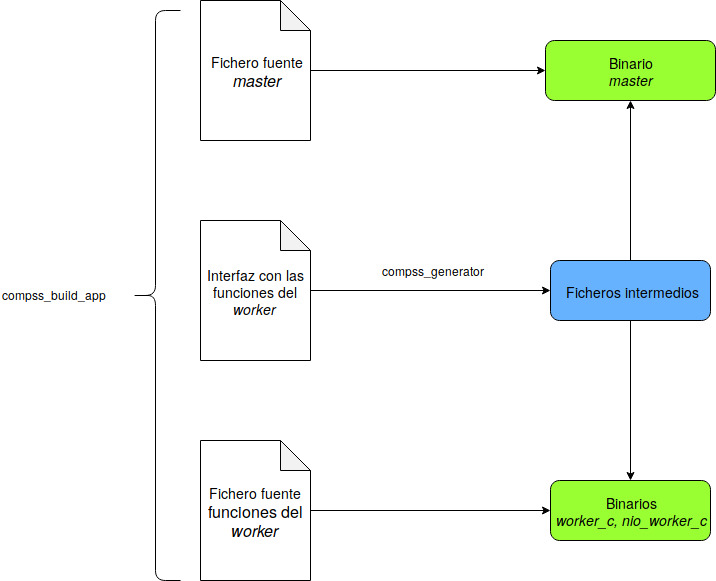
\includegraphics[width=\textwidth]{proceso_compilado.jpg}
    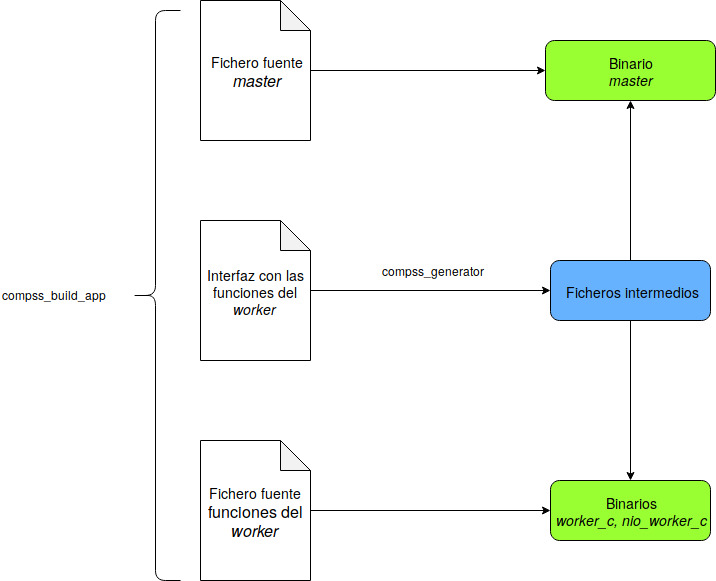
\includegraphics[scale=0.5]{proceso_compilado.jpg}
    \label{fig:proceso_compilado}
\end{figure}
\end{comment}

\subsubsection{Modelo de ejecución}

El modelo de ejecución es sencillo, muy similar al modelo \textit{thread-pool}, al iniciar el \textit{runtime} se levanta el \textit{master} y un conjunto de \textit{workers}, a medida que se vayan generando tareas se estudiará qué \textit{workers} están libres y si cumplen los requisitos para ejecutar dicha tarea, y en ese caso la ejecutarán. 

\begin{figure}[H]
    \centering 
    \caption{Modelo de ejecución, basado en la aplicación 'ejemplo'.}
    %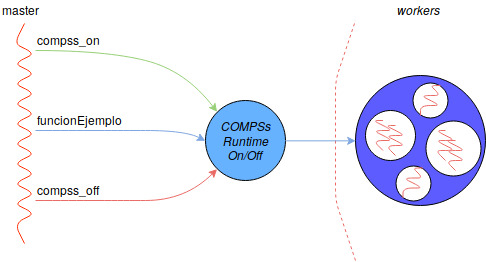
\includegraphics[width=\textwidth]{sta-masterworker.jpg}
    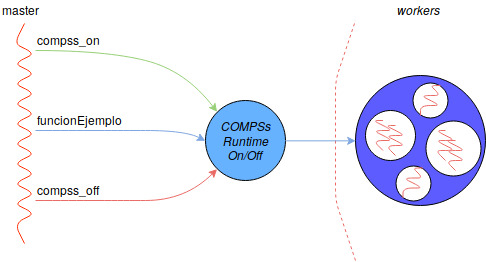
\includegraphics[scale=0.75]{sta-masterworker.jpg}
    \label{fig:masterworker_pool}
\end{figure}

La imagen muestra lo que sucede al ejecutar la aplicación de ejemplo de la sección \ref{compss_pm}, las líneas rojas curvas indican procesos (o bien \textit{threads}), lo importante sucede entre las flechas etiquetadas como compss\_on y compss\_off, la ejecución de la tarea. Se pide ejecutar la tarea funcionEjemplo al \textit{runtime} de \textit{COMPSs} y se decide en qué \textit{worker} se ejecutará. Hasta aquí podríamos pensar que es indéntico al \textit{thread-pool}, pero nótese la línea roja punteada que indica que los \textit{workers} no tiene por qué estar en el mismo nodo, por lo que en algún caso habría que enviar la tarea a otro nodo.
\par\bigskip

En \textit{C/C++} existen dos tipos de \textit{worker}, uno \textbf{no persistente} y otro \textbf{persistente}. 

\begin{itemize}
 \item \textbf{No persistente:} Para cada tarea que se quiere ejecutar en uno de estos workers se debe crear el \textit{thread} y unas \textit{pipes} para hacer \textit{Inter-process communication} (IPC). %No sé si indagar en qué se pasa por las pipes, hmmm... qué se pasa por las pipes?
 \item \textbf{Persistente:} Este tipo de \textit{worker} se levanta una vez al inicio de la aplicación y espera recibir las tareas a ejecutar.
\end{itemize}


\subsection{OmpSs}

\textit{OmpSs} es desarrollado por el grupo \textit{PM - Programming Models}, perteneciente también al departamento de \textit{CS - Computer Science}.
\par\bigskip

\textit{OmpSs} es un modelo de programación que intenta explotar el paralelismo de las aplicaciones de una manera sencilla y aprovechando al máximo los recursos de la máquina\cite{duran2011ompss}. 
\par\bigskip
El nombre del modelo proviene de \textit{OpenMP} y \textit{StarSs} (modelo que desarrolló el \textit{BSC}), este integra funcionalidades presentes en ambos. Por parte de \textit{OpenMP} se quiere tomar la facilidad de paralelizar una aplicación secuencial insertando pragmas, y de \textit{StarSs} el modelo de ejecución basado en un \textit{thread-pool} y que permite la ejecución de código en más recursos que únicamente el procesador, es decir, que ofrece fácil gestión del resto de recursos de cómputo (\textit{GPUs}, \textit{FPGAs}, ...)\cite{sainz2014leveraging}\cite{filgueras2013heterogeneous}.

\subsubsection{Modelo de programación y ejecución}

El modelo de programación de \textit{OmpSs} se basa en la generación de tareas sencillamente insertando pragmas en código secuencial y a su vez facilitando la gestión de recursos heterogéneos. Veamos un pequeño ejemplo que muestre estas facultades.

\begin{lstlisting}[caption={Multiplicación de un bloque de una matriz utilizando GPUs.}, captionpos=b, label={lst:ejemplo-functions.cc}, language=C++]
for (int i = 0; i < N; ++i) {
    for (int j = 0; j < N; ++j) {
        for (int k = 0; k < N; ++k) {
            #pragma omp target device(cuda) \
                               copy_deps    \
                               ndrange(2,N,N,32,32)
            #pragma omp task inout([N*N]C) in([N*N]A, [N*N]B)
            multiply_partitions_GPU(A[i*N+k], 
                                    B[k*N+j], 
                                    C[i*N+j], 
                                    n);
        }
    }
}
\end{lstlisting}

El código muestra una multiplicación de matrices por bloques. Con el primer pragma se indica que el dispositivo objetivo es una tarjeta gráfica que soporte \textit{CUDA}, y el segundo la declaración de una tarea y el tamaño de los bloques junto a las dependencias de esta.
\par\bigskip

El modelo de ejecución consiste en un \textit{thread-pool}, es decir, al generar tareas se escogerán \textit{threads} del \textit{pool} (entendámoslo como un conjunto de \textit{threads}) para ejecutarlas.
\par\bigskip

Cabe decir que para compilar una aplicación de \textit{OmpSs}, se utiliza el compilador \textit{source-to-source Mercurium} y el runtime \textit{Nanos++} para gestionar el paralelismo, es decir, la creación de tareas, sincronización entre estas, etc.

\subsection{COMPSs+OmpSs} \label{compssompss}

Actualmente existe la posibilidad de desarrollar aplicaciones que utilicen \textit{OmpSs} dentro de \textit{COMPSs}. 
\par\bigskip
Para poder interactuar con el \textit{runtime} de \textit{OmpSs} \textit{Nanos++}, necesitamos gestionarlo nosotros manualmente o bien utilizar los pragmas que nos propone el modelo de programación y compilar con \textit{Mercurium}. Entonces, asegurándonos de registrar los \textit{workers} en el \textit{runtime} y compilando su código fuente con \textit{Mercurium} aseguramos la interacción con el \textit{runtime} y por lo tanto la integración de ambos modelos.

Es posible desarrollar aplicaciones, como ya se ha comentado, pero con ciertas restricciones. Las problemáticas aparecen con los dos tipos de \textit{worker} que hemos visto antes. Para el worker no persistente, no suele valer la pena debido a la granularidad de las tareas de \textit{OmpSs}. El \textit{overhead} proviene de crear el \textit{thread} del \textit{worker}, registrarlo en el \textit{runtime Nanos++} y levantar las \textit{pipes}. El persistente carece del \textit{overhead} de levantar las \textit{pipes} y el resto, vale la pena ya que el \textit{worker} persiste durante la ejecución de la aplicación. Pese a que el persistente mejora respecto al no persitente, hay problemas de migración de \textit{threads} entre aplicaciones cuando se ejecutan varias a la vez.
\par\bigskip

Estos problemas pretenden arreglarse integrando \textit{OmpSs-2}, que ofrece un \textit{runtime} nuevo llamado \textit{Nanos6} y nuevas características que vienen con este cambio como por ejemplo:

\begin{itemize}
\item \textbf{Liberación de las dependencias:} Las dependencias en esta versión se liberen de manera temprana, es decir, una vez una tarea acaba con un dato lo notifica al \textit{runtime} y este se encarga de notificar a las tareas que quedan libres de esta dependencia.
 \item \textbf{Relajación de las dependencias:} Ahora se pueden utilizar nuevos pragmas para determinar dependencias más suaves, no tan estrictas como en la versión anterior.
 \item \textbf{Ejecución de funciones de manera asíncrona:} La \textit{API} del nuevo \textit{runtime} \textit{Nanos6} permite ejecutar de manera asíncrona funciones en forma de tarea a partir de un puntero a una función.
\end{itemize}

Hemos listado las que de alguna manera eran clave para el proyecto, \textit{OmpSs-2} implementa muchas otras mejorías a parte de estas\cite{OmpSs2reference}. Una vez integrado, el proyecto estudiará si realmente han sido solucionadas las problemáticas anteriormente planteadas.

\section{Alcance del proyecto}

En esta sección se declaran las intenciones del proyecto (qué se pretende hacer), mediante una serie de requerimientos que harán que el proyecto pueda ser acabado con éxito, y unos objetivos que marcarán el desarrollo de este. También los posibles riesgos que surjan (y las soluciones de estos) y la metodología de trabajo que se llevará a cabo.

\subsection{Requerimientos}

 Los requerimientos necesarios para este proyecto son:

\begin{itemize}
 \item La nueva integración con \textit{OmpSs-2} no debe romper la actual compatibilidad con \textit{OmpSs}.
 \item El rendimiento de las aplicaciones desarrolladas con \textit{COMPSs+OmpSs-2} debe mejorar.
 \item Todas las modificaciones sobre \textit{COMPSs} deben ajustarse al grupo de \textit{Workflows and Distributed Computing}.
 \item Cualquier requerimiento impuesto (o aconsejado) por el \textit{BSC} formará parte de esta lista.
  
\end{itemize}

\subsection{Objetivos}

El objetivo principal de este proyecto es reformular la integración de \textit{COMPSs} con \textit{OmpSs} para solucionar los problemas actuales, ya sea integrándolo de nuevo pero esta vez con \textit{OmpSs-2} o bien idear otra manera de resolver las problemáticas. La siguiente lista muestra la posible descomposición de objetivos:

\begin{itemize}
 \item Aprender a utilizar la API (\textit{Application Programming Interface}) de \textit{Nanos6}.
 \item Eliminar o bien reducir las problemáticas planteadas en la sección   \ref{compssompss}.
  \item Mejorar la gestión de recursos heterogéneos en las aplicaciones desarrolladas en \textit{COMPSs} integrando \textit{OmpSs-2}.
 \item En caso de conseguir el resto de objetivos plantear la integración en \textit{Java} y \textit{Python}.
\end{itemize}

\subsection{Riesgos}

Durante el desarrollo del proyecto pueden surgir problemas, para mejorar la reacción ante ellos listaremos los posibles riesgos y las respectivas soluciones.

\subsubsection{Problemas con el material de desarrollo}

Se podría romper el equipo en el cual se desarrolla el proyecto, pongamos que de una pantalla, un teclado y un ordenador se rompe el último. Se perdería todo el avance del proyecto, incluso documentación.
\par\medskip

\textbf{Solución:} Pese a que la pérdida del ordenador es importante, todo el código del proyecto será subido al \textit{GitLab} de \textit{WDS}, y la documentación al \textit{GitHub} personal del desarrollador, por lo cual se podría recuperar todo el  proyecto.

\subsubsection{Problemas con los clústers y supercomputadores}

Si por casualidad, caen los clústers y supercomputadores en los cuales se medirá el rendimiento del proyecto, se pararía la obtención de las métricas. 
\par\medskip

\textbf{Solución:} En este caso, como no resultaría lo mismo ejecutarlo en local en mi ordenador, debería optar por realizar otras tareas hasta que el equipo del \textit{BSC} solucione los inconvenientes.

\subsubsection{Aparición de errores en la implementación}

Cualquier proyecto esta lleno de errores en la implementación, hay que saber encontrarlos y solucionarlos lo más rápido posible, pero puede entorpecer el proyecto.
\par\medskip

\textbf{Solución:} Activaremos los \textit{flags} de \textit{debug} para poder evitar el mínimo error y en caso de su aparición utilizaremos \textit{gdb} (\textit{GNU Debugger}) para encontrarlo.

\subsubsection{Problemas con OmpSs/OmpSs-2}

Dado que se realizará una integración de otro proyecto del \textit{BSC} el desarrollador puede encontrarse con dificultades relacionadas con este a lo largo del proyecto.
\par\medskip

\textbf{Solución:} Después de haber intentado solucionarlo por sus propios medios se pondrá en contacto con el grupo de \textit{Programming Tools} con la descripción del error e intentos de solucionarlo.

\section{Metodología}

Para decidir la metodología a utilizar, hay que tener en cuenta que el proyecto consta únicamente de tres personas que se envolverán en él. El desarrollador, que hará todo el desarrollo tangible, el director y el codirector. 
\par\bigskip

La metodología que más se ciñe a las características del ``equipo'' es \textit{SCRUM}. Esta metodología forma parte de las populares (y bastante de moda) metodologías ágiles, consiste en planear al milímetro las tareas a realizar, y hacer una predicción de qué se conseguira hacer y que no en cortos periodos de tiempo llamados iteraciones. Además de estas predicciones, se consultará el estado del proyecto a diario, con cuestiones como ``¿Desde la última reunión que he conseguido?'', ``¿Desde entonces que haré para llegar a los objetivos de la iteración?'', ``¿Algún impedimento que no me permita alcanzar estos objetivos?''.
\par\bigskip

Esta metodología nos permitirá reaccionar rápidamente a los imprevistos, además de hacer un bueno monitoreo del estado del proyecto, por lo cual se ha decidido emplearla.

\subsection{Herramientas}

Para efectuar el seguimiento del proyecto junto a mi director y codirector, se empleará un \textit{workspace} de \textit{Slack} para las comunicaciones directas (decidir dónde y cuándo hacer las reuniones por ejemplo), y \textit{Trello} para gestionar las tareas a desempeñar en cada iteración. Como ya se ha mencionado anteriormente, para el control de versiones del proyecto, código y documentación se utilizará respectivamente \textit{GitLab} y \textit{GitHub}.
